\chapter{Dynamic Programming}
Transforming complex problems into a sequence of subproblems whose solutions can be used to construct a solution for the bigger and original problem.
It also is a general framework for analyzing and solving optimization problems effectively and fast\footnote{Usually optimization problems require exponential time to be solved.}.

Dynamic programming decompose large problem in a collection of small problems which can be solved in linear order (forming a implicit conceptual DAG) one after the other, from the \textit{smallest} to the \textit{largest} and using solution to the small ones to solve the bigger ones. 

\section{DAG shortest Path}
Probably one of the easiest example that can depict the concept behind DP is the problem of computing the shortest path in a DAG (because of the analogy with DP itself which linearize problems and the fact that DAGs can be linearized s.t. all the edges point forward).

\begin{framed}
A DAG is a graph such that exists a topological ordering (see figure \ref{fig:DAGsort}) of nodes $v1,v2, \ldots,v_n$ (we assign an differen interger to each  node) s.t. for each edge $(i,j)$ we have that $i<j$.
	
\end{framed}

	\begin{figure}
	\label{fig:DAGsort}
	\centering
	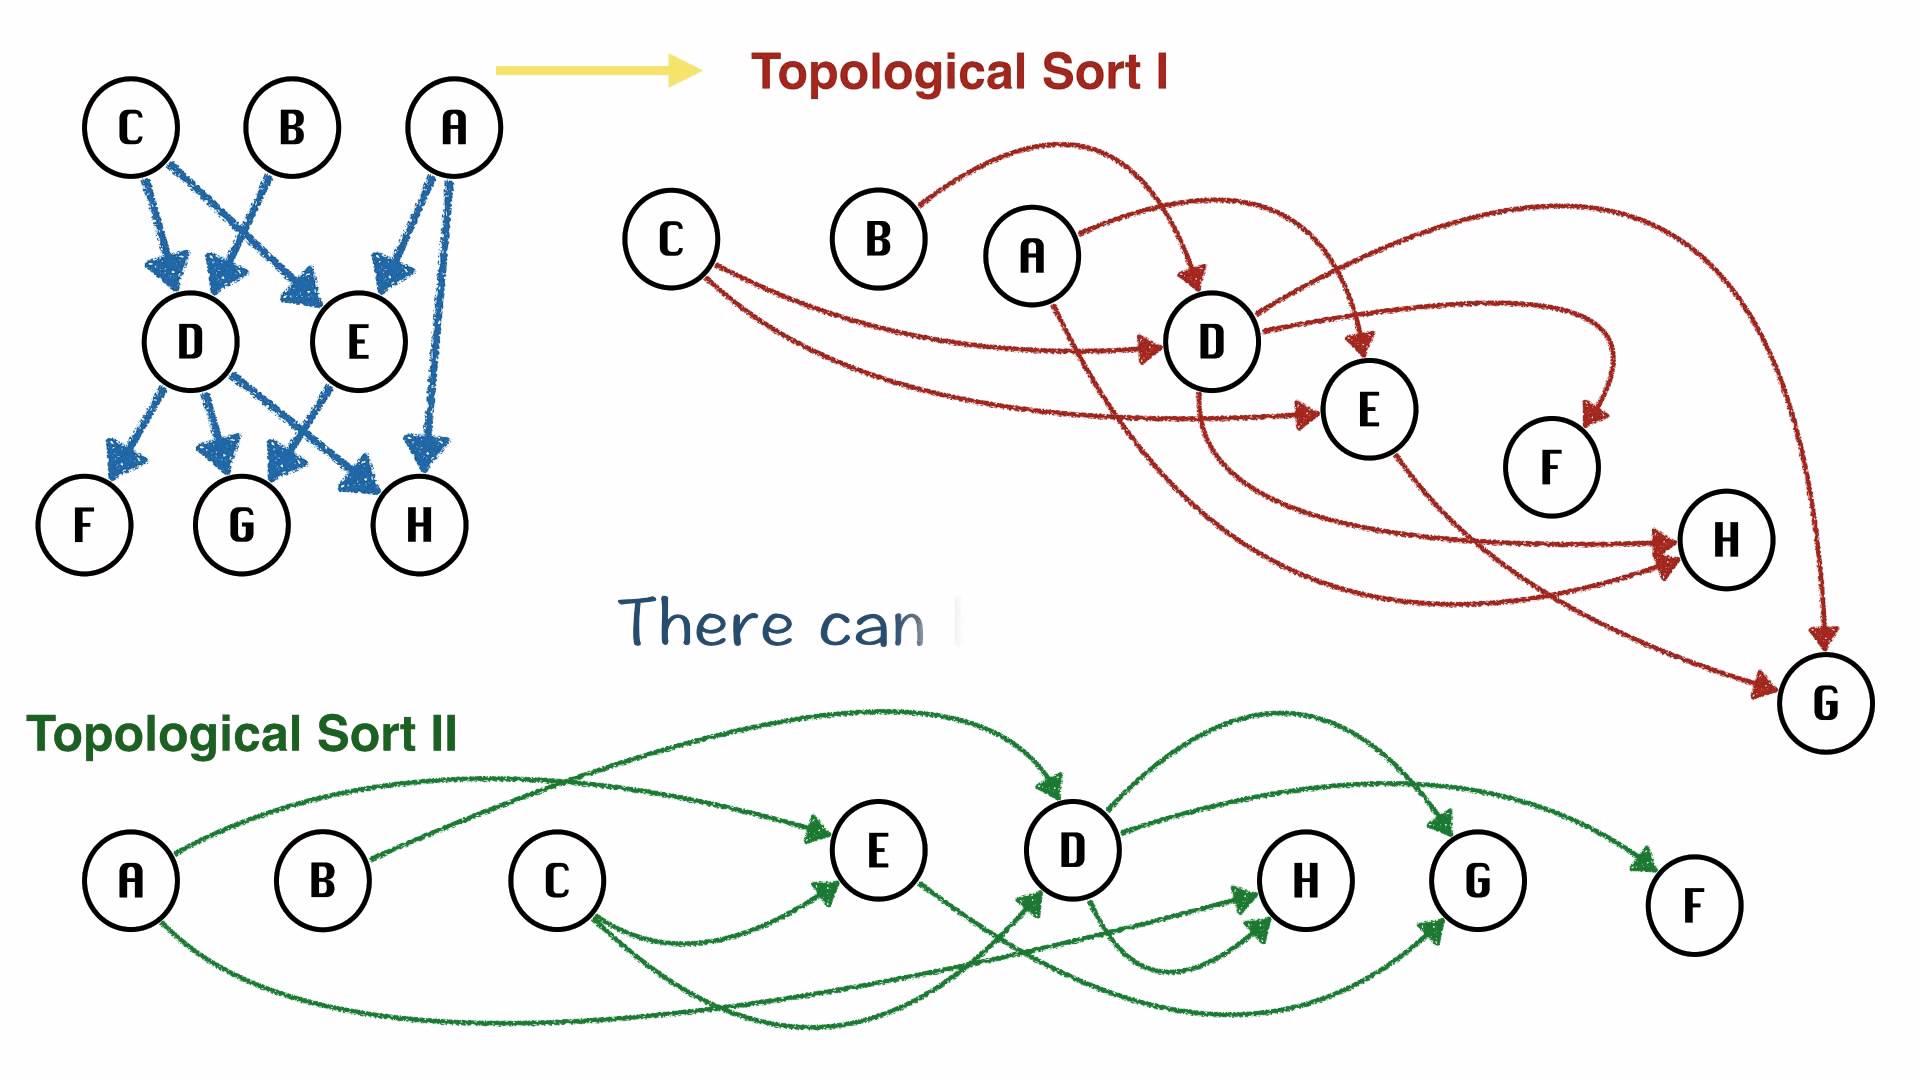
\includegraphics[width=\textwidth]{../images/DAGsort}
	\caption{DAG topological sorting}
	\end{figure}


Problem here is to find the shortest (largest works fine as well) between a two nodes $s$ called source and $d$ destination.
Consider, the DAG in figure \ref{fig:dagexample} with $s=A$ and $d=E$
	\begin{figure}
	\label{fig:dagexample}
	\centering
	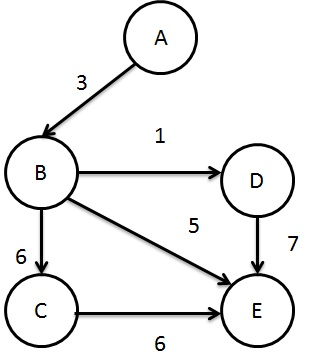
\includegraphics[width=0.5\textwidth]{../images/dagexample}
	\caption{DAG topological sorting}
	\end{figure}
In order to compute the shotest path it is usefult to think as follows. We know that any possible path that leads to $E$ eventually has to go through ieither $C,B,D$ cause those are the only edges that point inwards to $E$, out destination.
Is like willing to go to Rome which has three roads only  from outside the city to the center.
The length of the shortest path is clearly the following:
\[
	dist(A,E) = min\{dist(A,D)+weigth(D,E), dist(A,C)+weigth(C,E), dist(A,B)+weigth(B,E)\}
\]
As one can see from the above expression this formulation is made up of 3 smaller subproblems which can be solved the same way as the bigger problem.
One can ask the question, how much does the shortest path between $A$ and $D$ weights? Well it is formulaed the same way (ansering the question, how many inward edges $D$ has?):
\[
dist(A,D) = min\{dist(A,B) + weight(B,D)\} = dist(A,B) + weight(B,D)
\]
The nice thing about this approach is that if we work our way from A to E in a left to right manner (assuming DAG topological order) at time of computing any \textit{dist} subproblem we already have computed all relevant subproblems that allow us to solve the particular istance at hand (proceeding this way until we have solved all the subproblems).
A simple schematization of this ideas lead us to the pseudocode in listing (\ref{alg:dagshortest})
\begin{algorithm}\label{alg:dagshortest}
\Fn{DAG\_SHORTEST (A,E)}{
	\For{$i \gets 1$ \textbf{to} $n$} {
		$dist(A,n) \gets \infty$;
	}
	$dist(A,A) \gets 0$;\\
	\For{$v \in V \setminus\{A\}$ \texttt{in linearized order} }{
		$dist(A,v) \gets \min_{(u,v) \in E}{dist(A,u) + weight(u,v)}$
	}
}
\caption{DAG shortest path algorithm}
\end{algorithm}
Start at the very right. Distance from source to source is obviously zero, you don't need to move at all. 
Next node taken in consideration is (because they are linearly ordered) is $B$ for which the only edge having it as second node is $(A,B)$. Shortest path to 
$B$ is then $dista(A,A)=0 + weight(A,B) =3$ which totals $3$. Next ones is $C$ which has only one edge leading into it, $(B,C)$. $dist(A,C) = dist(A,B) + weight(B,C) = 3+6=9$.
Next one is $D$, again only one edge leading into it, $(B,D)$ which allows us to compute its shortest path from A: $dist(A,D) = dist(A,B) + weight(B,D) = 3 +1 =4$.
Next one is $E$ our destination node which has the following inwards edges $\{(D,E),(B,E), (C,E)\}$.Shortest path from $a$ to $E$ is then 
the minimum among the following quantities:
\[
	dist(A,B) + weight(B,E) = 3+5=8
\]
\[
	dist(A,C) + weight(C,E) = 7 + 9 = 16
\]
\[
	dist(A,D) + weight(D,E) = 2 +7 =9
\]
Minimum among $5,13,9$ is $5$ which happens to be the shortest path weight between $A$ and $E$ in graph in figure \ref{fig:dagexample}.
Is important to note here that we haven't find the actual \textit{path} but rather the weith of one of the possible shortest path! In order to find the shortest path we need to do some more work and record at each step i.e. at each subproblem solved or in other words when we find an intermediate shortest path value which is the parent node for which happen that the distance is minimal (Among all the inwards edges which one leads to the minimum weight?).
We will record all this informations in an associative array, \textit{parent}:
In the previous example when solving $dist(A,B)$ we found out that the shortest path was hopping through node $A$:  parent[B] = A;
For node $C$ shortest path was going through node B so parent[C] =B;
For node $D$ shortest path was going through node B so parent[D] =B;
For node $B$ shortest path was going through node B so parent[E] =B;
We can work the path backwards from the destination node and reconstruct all the hops using the \textit{parent} relationship.
$path(A,E) = E \rightarrow parent(E) \rightarrow  parent[parent[E]] \rightarrow  \ldots \rightarrow $ until we reach the souce node.
\section{Practice Problems}

\subsection{Longest Increasing Subsequence}
The longest increasing subsequence is the problem of finding a subset $V_a=v_{a_1} \leq v_{a_2} \leq\ldots \leq v_{a_k}$, $a_1 < a_2 < \ldots < a_k$ and not other subsequence $V_b=v_{b_1}\leq v_{b_2}\leq \ldots \leq v_{b_l}$, $b_1 < b_2 < \ldots < b_l$ s.t. l > k.

The solution to this problems has to be a sequence of any size of element of the original collection s.t. the its overlall sum is \textbf{maximal}.

The naive approach leads to a $\Theta(2^n)$ algorithm which considers possible subset. Since there are an exponential number of such subsets this leads to a \textbf{exponential algorithm}.
We can do much better using DP.
Our goal is to recursively formulate the solution in terms of smaller problems than have no dependencies at all with the bigger ones.  Using the DAG analogy this means that for each subproblem to be solved the only information needed are solution to even smaller subproblems.

Let's work our way from the end of the array. What we know for sure is that the last element of the array can't be itself the first of a subsequence longer than one.
What we know about the second last element?
If a subsequence starts at this location then its lenght may be one or two depending weather this element is greater or less then the last one.
What about the third last? Again any subsequence starting at this location may be of lengths $1,2,3$ depeding weather it is greater than both the subsequent ones or only of one of them (no matter which one) or lesser than both.
This lead us to the following statement. Working our way backwards, at each location $i$ the longest subsequence starting at $i$ is the longest subsequence starting at any index greater than $i$ s.t. $V[j] > V[i]$ , $j>i$ i.e. the next element must be greater than the element at index $i$ (after all we are trying to find an increasing subsequence). 
Generalizing this idea we can formulate the solution as follows:
\[
LS(n) = 1+ \underset{ \underset{ V[i] > V[n]}{i > n} }{\max}{ LS[i]}
\]
 
In order to solve this problems we have created a list of subproblems with the following properties:
Problems are orderable and there exists a dependence between bigger and smaller problems. Bigger problems depends only on smaller problems, smaller problems depends on even smaller problems and so on until we reach the base case for which we already know the answer or we can compute it withoth using any other subproblem at all.
Each subproblem requires is dependent not only on one (smaller) subproblem but on all the smaller subproblems (the max operator iterate all subproblems till the base case)!
The complexity of solving one subproblem is then the complexity of finding the maximum value in a collection of values which can be done in $O(n)$. since we have to solve $n$ of this subproblems the complexity is quadratic $O(n^2)$. It is important to note that the max operator takes linear time \textbf{only} is we remember the solution to the smaller problems without recomputing them all the times they are required to be solved. This \textit{remembrance} is called \textbf{memoization} and is a key concept in \textbf{dymanic programming}. \textbf{Solution to problems that are required to be solved over and over have to be memoized}. 
Problems that exposes this pattern of decomposition i.e. that requires subproblems to be solved over and over again are said to have the property of \textbf{overlapping subproblems}. Memoization skyrocket the algorithm when a problem has this property.
The following is the pseudocode for the \textit{longest increasing subsequence}.

\subsection{Longest Common Subsequence}
The longest common subsequence problem deals with the problem of finding two subsequence (which are not contiguous characters, those are called substrings) from two strings $A,B$ s.t. their size is maximixed. 
A naive algorithm would simply list all possible subset $a_i$ of $A$ ($\Theta(2^n)$) and for each of them it would test whether it is present in $B$ (cost is ($O(n)$ time).
We can do much better using dynamic programming. It isnot hard to come up with a memoization-ready definition of the longest common subsequence that will allow us to decrease the complexity of the from the naive exponential to quadratic.


Let's note that a LCS a string of length $0$ and any other string is easy to compute, since it is always $0$. This will be our base case.
Let's denote $LCS(i,j)$ the solution to the problem using only characters of $A$ up to $i$ and of $b$ up to $j$. 
Now, if $A[i] = B[j] $ the LCS(i,j) is equal to $1+LCS(i-1,j-1)$ since any solution to smaller subproblems can be improved by adding one, corresponding to the element $A[i]$ and $B[j]$.
Consider the case where $A=aabb$ and $B=abab$. $LCS(4,4) = 1+LCS(3,3)$ since any common subsequence (hence the longest as well) can be enlonged with the last $b$ (which is clearly common between the two strings).

Now consider the case where $A=aabb$ and $B=abaa$ and $A[4]=a \neq  B[4]=b$. A common subsequence clearly does not involve those two characters but it could involve just one of them with one of smaller index (for example $A[4] = B[2]$). We have two cases then, $LCS(i-1,j)$ and $LCS(i,j-1)$.
Our algorithm is then the following:
 \begin{algorithm}\label{alg:dagshortest}
\Fn{LCS (i,j)}{
	\If{$i\leq 0$ \textbf{or} $j\leq 0$}{
		\Return $0$ \;
		}
	\If{$A[i]=B[j]$}{
		\Return  $1+LCS(i-1,j-1)$\;
	}
	\Return $max(LCS(i-1,j),LCS(i,j-1))	$\;
		
}
\caption{Longest common subsequence}
\end{algorithm}
This algorithm is still exponential since in the worst case it call itself twice at each call. Since the possible values for the pairs $i,j$ is quadratic this is a good hint for thinking about memoization. It means that a lot of smaller subproblems are solved multiple time. This is again the property of overlapping subproblems. Memoization will decrease the complexity to a more reasonable $O(nm)$ where $n$ and $m$ are the length of the two strings. Note how this approach can easily extended to longest common subsequence over $k$ strings. The complexity will be $\prod_i^k n_i$ where $n_i$ is the length of the $i^th$ string.

The bottom up approach is very similar. 


\subsection{Maximum Sum Contiguous Subsequence}
Given a sequence of n real numbers $A(1) \ldots A(n)$, determine a contiguous subsequence A(i) ... A(j) for which the sum of elements in the subsequence is maximized.



\subsection{Minimum Steps to One}
Given an integer $n$ and three operation that can be performed on it find the minimum number of operations needed to get $1$. Tne available operations are
\begin{enumerate}
\item Subtract one. $n_{i+1}=n_{i}-1$
\item Divide by two. If n is divisible by two then $n_{i+1}=\frac{n_{i}}{2}$
\item Divide by three. If n is divisible by three then $n_{i+1}=\frac{n_{i}}{3}$
\end{enumerate}

	The main idea is to store for each number less than $n$ the minim value it takes to reach $1$. Tbe base case is trivial and is $1$ which takes $0$ steps.
	We can iterate over all the number is a botto-up fashion in the following manner
	
	\begin{algorithm}\label{alg:dagshortest}
\Fn{MSTO(N)}{
	$T[1] = 0$\;
	\For{$i \gets 2$ \textbf{to} $N$} {
		$m \gets T[i-1]$\;
		$dtwo \gets \infty$\;
		$dthree \gets \infty$\;
		\If{$i\%2==0$}{
					$dtwo \gets T[\frac{i}{2}]$\;			
		}
		\If{$i\%3==0$}{
			$dthree \gets T[\frac{i}{3}]$\;			
		}
		$T[i]=1+min(m,dtwo,dthree)$\;
	}
	
}
\caption{DAG shortest path algorithm}
\end{algorithm}
For each number less than $n$ we basically answer the following question: the best way to transform $n$ into $1$ checking in which, using the available operation, number we can trasnform $n$ at a cost of one operation that yeld to the minimum numeber of operation. 

The top-down memoization problem uses the following recursive definition
\[
	MSTO(N) = min(MSTO(n-1),m2,m3))
\]
where $m2$ is $MSTO(\frac{n}{2})$ if $n$ is divisible by two and m3 is defined similarly. Tne key idea here is again, memorization. We should recognize that the overlapping problem property holds because different branches may end up computing the same sub-problem. We solve this issue by storing all partial results in a table for no longer compute any subproblem.
Since we do atual computation only for \textbf{new} number, than the complexity is linear in $n$.  This analysis is much simpler if we look at the bottom-up version of the solution.

\subsection{Binary Knapsack}
Given a set list of $n$ items $P=\{p_1,p_2,\ldots,p_n\}$ with a weight  $w_i$ and a value $v_i$ associated with them, a maximum knapsack capacity $W$ find the subset of $P$
s.t. the sum of the values is maximal and the sum of the weights is less or equal than $W$.

We could be tempted to start thinking in a greedy way i.e. sort the element by their value and start putting them into the knapsack one after the other until the bag is full or no other elements can be stored. This approach can give us reasonable good solution in many cases but it does not garantee that it find the optimal solution!
As an example consider the following list of elements $(w_i,v_i)$, $P=\{p_0=(8,10),p_1=(3,5),p_2=(3,4),p_3=(3,2),\}$. The greedy approach will first put the element $p_0$ into the bag since it has the best value, leaving no space for the remaining elements (altough the bag is still $20\%$ empty for a total value of $10$. A better solution would include the following elements: $p_1,p_2,p_3$ with a total value of $11$.

Let's try to solve it out using DP. We have to be able to write the solution as a recurrence formula in which all the recurrent part refer to subproblems.
We define $S(i,W)$ as being the solution of the knapsack problem using  all but the last $i$ elements and $W$ is the current weight constraint.
\[S(i,V,W) = \left\{
  \begin{array}{lr}
    0  &: i \leq 0 \; \mbox{or} \; W\leq 0\\
    S(i-1,V,W) &: w_i > W \\
    \max(S(i-1,W),S(i-1,V+v_i,W-w_i))
  \end{array}
\right.
\]
The previous formula states that if the collection of elements is empty or the space into the bag is zero then the maximum value possible is simply zero.
The second rule says that is the element number $i$ is heavier than the current available space then this element cannot be taken so is skipped.
The third one states that the maximum amount can be get by either include the item $i$ into the solution or not. 

\begin{lstlisting}[language=c++, caption="Binary knapsack problem - exponential",label=list:knapexp]

int solveKnapsack(int V, int W, int i){
    if(W<=0 || i<0)
        return V;
    int v = solveKnapsack(V,W,i-1);
    int v1 =-1;
    if(weights[i] <= W)
       v1= solveKnapsack(V+values[i],W-weights[i],i-1);
        
    return max(v,v1);
    
}

	\end{lstlisting}

Whsat is the running time of this algorithm? Well as it is coded in listing \ref{list:knapexp} the running time is exponential because overlapping subproblems are recomputed many times.
Since we systematically check weather each element can be or cannot be in the final solution this yelds to a $O(2^n)$ solution.
We should first notice that there are not so many different subproblems cause $W$ and $i$ are the only parameters that define a subproblem. This means that there are only $W \times n$ different subproblems. This means that we recompute an exponential number of times the same set of subproblems. Solution is given by memoization. 

The listing \ref{list:knapqudratic} shows how to improve the listing \ref{list:knapexp} with memoization to achieve $O(W n)$ complexity.


\begin{lstlisting}[language=c++, caption="Binary knapsack problem -Memoized solution",label=list:knapqudratic]
int solveKnapsackQ(int V, int W, int i){
    if(T[i+1][W] !=-1)
        return T[i][W];
    if(W<=0 || i<0)
        return V;
    
    int v = solveKnapsackQ(V,W,i-1);
    int v1 =-1;
    if(weights[i] <= W)
       v1= solveKnapsackQ(V+values[i],W-weights[i],i-1);
    
    T[i+1][W]= max(v,v1);
    return T[i+1][W];
}
	\end{lstlisting}

To get an idea on the difference of computation time between the two verions lets try to run the two example on the same dataset (not incredibly large afterall, $n=30$). You can generate the used output using the following bash commands:

\begin{lstlisting}[language=c++, caption="Binary knapsack problem -Input generation",label=list:knapqudratic]
	echo "30 100" > test.txt	
	seq -s" " 30 -1  1 >> test.txt 
    seq -s" " 30 1 >> test.txt 
\end{lstlisting}
The input file contains three lines. The first one contains two integers $n$ and $W$ respectively.
The two subsequent lines contain $n$ lines each, values and weights.

Write a simple main, and run the two knapsack solution we have provided in this section (I suggest you to go for a coffee during the execution of the exponential one).


\subsection{Rod cutting}
This is a classical DP problem in which we have to maximize our profit from cutting a rod of length $n$ into smaller parts.
The number $p[i]$ identifies the profit given from a part of length $i$. Obviously $1 \leq i \leq n$ since we cannot have a rod of length $0$ or one of length greater than $n$.
Goal of the problem is to find the best set of cuts s.t. the sum of the profits obtained from all the cuts is maximixed.
As an example imagine to have a rod of length $8$ and lengths profits as in table \ref{rodcut}. The optimal solution consists in cutting the original rod into 2 smaller rods, of size $2$ and $6$ respctively. 
\begin{table}[]
\centering
\caption{Rod cutting lengths profits}
\label{rodcut}
\begin{tabular}{lllllllll}
 1&  2&  3&  4&  5&   6&   7&  8&\\
 1&  5&  8&  9&  10&  17&  17& 20& 
\end{tabular}
\end{table}
A naive approach in solving this problems would require to generate all possible way we can cut a rod of length $n$. The number of ways we can cut a rod of length $n$ using in smaller parts is equivalent to the number of partitions of $n$ which is exponential in $n$.

Again dynamic programming comes to help. We just need to notice how this problem satisfies the two properties of dynamic programming:
\begin{enumerate}
\item Optimal Substructure
\item Overlapping Subproblem
\end{enumerate}
Regarding optimal substructure, imagine that an oracle tells you that the first cut in the optimal solution is $k\leq n$. Then solution is obtanible simply by solving the same rod cutting problem but with a smaller problem i.e. $n' = n-k$. 
This is called optimal substructure, the property s.t. solution to a problem depends on optimal solution of smaller subproblems!

This allows us to define to rod cutting solution as the following recurrence relation:
\[
RC(N) = \max_{0\leq i\leq N-1} P[i] + RC(N-i)
\]
From this we can deduce that this solution also have the property of overlapping subproblems (It is sufficient to draw the call tree for a small $N$ to notice it).
So this is a perfect candidate for dynamic programming.
Following is a top down with memoization implementation.
\begin{lstlisting}[language=c++, caption="Binary knapsack problem -Memoized solution",label=list:knapqudratic]
int solveCuttingRod(int N, int* price,int* memo) {
    if(N==0)
        return 0;
    if(memo[N-1]!= -1)
        return memo[N-1];

    int m = INT_MIN;
    for(int i=1; i<=N; i++)
        m = max(m,price[i-1]+solveCuttingRod(N-i,price,memo));

    memo[N-1]=m;
    return m;
}

	\end{lstlisting}
Since each problem is solved exactly once (because subseauent calls are handled by the memoization table) and each call does a linear work this mean that this approach has complexity $\Theta(n^2)$ which is a very good improvement from the exponential naive solution!


